\documentclass[conference]{IEEEtran}
\usepackage{amsmath,amssymb,amsfonts}
\usepackage{xcolor}
\usepackage{tikz}
\usepackage{amsmath,amssymb,braket}
\usetikzlibrary{decorations.pathreplacing,calc}

\begin{document}

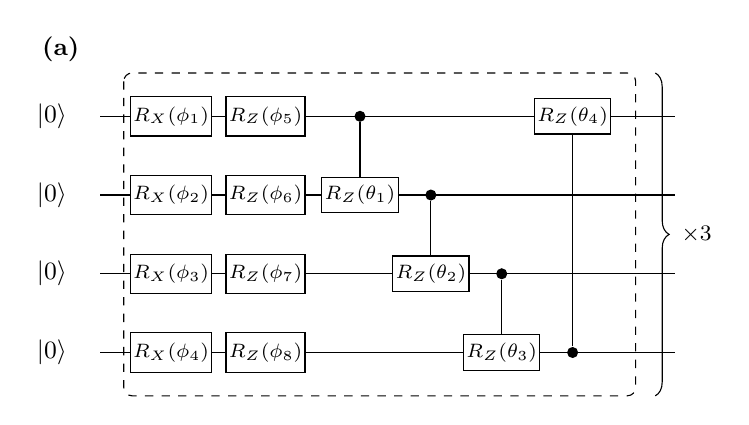
\begin{tikzpicture}[
    gate/.style={draw, fill=white, minimum width=0.9cm, minimum height=0.5cm, 
                 font=\scriptsize, inner sep=1pt},
    rzbox/.style={draw, fill=white, minimum width=0.85cm, minimum height=0.45cm, 
                  font=\scriptsize, inner sep=1pt},
    ctrl/.style={fill=black, circle, inner sep=0pt, minimum size=4pt},
    targ/.style={draw, circle, inner sep=0pt, minimum size=8pt, line width=0.4pt,
        path picture={
            \draw[line width=0.4pt] 
                (path picture bounding box.south) -- (path picture bounding box.north);
            \draw[line width=0.4pt] 
                (path picture bounding box.west) -- (path picture bounding box.east);
        }
    }
]

% ================================================================
%  Circuit 2 — CRZ Ring
% ================================================================
\def\yoff{-5.0}

\node[font=\small\bfseries] at (0.3, 0.85+\yoff) {(a)};

\foreach \i in {0,...,3} {
    \pgfmathsetmacro{\ypos}{\yoff - \i}
    \node[left, font=\small] at (0.5, \ypos) {$\ket{0}$};
    \draw (0.8, \ypos) -- (8.1, \ypos);
}

% RX gates — now phi
\node[gate] at (1.7, \yoff)   {$R_X(\phi_1)$};
\node[gate] at (1.7, \yoff-1) {$R_X(\phi_2)$};
\node[gate] at (1.7, \yoff-2) {$R_X(\phi_3)$};
\node[gate] at (1.7, \yoff-3) {$R_X(\phi_4)$};

% RZ gates — now phi
\node[gate] at (2.9, \yoff)   {$R_Z(\phi_5)$};
\node[gate] at (2.9, \yoff-1) {$R_Z(\phi_6)$};
\node[gate] at (2.9, \yoff-2) {$R_Z(\phi_7)$};
\node[gate] at (2.9, \yoff-3) {$R_Z(\phi_8)$};

% CRZ ring — theta for entangling parameters
\node[ctrl] (c2a) at (4.1, \yoff) {};
\node[rzbox] (t2a) at (4.1, \yoff-1) {$R_Z(\theta_1)$};
\draw (c2a) -- (t2a);

\node[ctrl] (c2b) at (5.0, \yoff-1) {};
\node[rzbox] (t2b) at (5.0, \yoff-2) {$R_Z(\theta_2)$};
\draw (c2b) -- (t2b);

\node[ctrl] (c2c) at (5.9, \yoff-2) {};
\node[rzbox] (t2c) at (5.9, \yoff-3) {$R_Z(\theta_3)$};
\draw (c2c) -- (t2c);

\node[ctrl] (c2d) at (6.8, \yoff-3) {};
\node[rzbox] (t2d) at (6.8, \yoff) {$R_Z(\theta_4)$};
\draw (c2d) -- (t2d);

\draw[dashed, rounded corners=3pt] (1.1, 0.55+\yoff) rectangle (7.6, -3.55+\yoff);

% Brace — direction flipped (no mirror)
\draw[decorate, decoration={brace, amplitude=5pt}] 
    (7.85, 0.55+\yoff) -- (7.85, -3.55+\yoff) 
    node[midway, right=6pt, font=\footnotesize] {$\times 3$};
\end{tikzpicture}

\end{document}